\documentclass[border=8pt,12pt]{standalone}
\usepackage{times}
\usepackage{roboto}
\usepackage{inconsolata}
\usepackage[T1]{fontenc}
\usepackage{amsmath,amssymb,xcolor}
\usepackage{tikz}
\usetikzlibrary{arrows.meta, positioning, shadows}
\newcommand{\hdr}[1]{{\robotoslab\fontseries{l}\selectfont\LARGE #1}}
\begin{document}
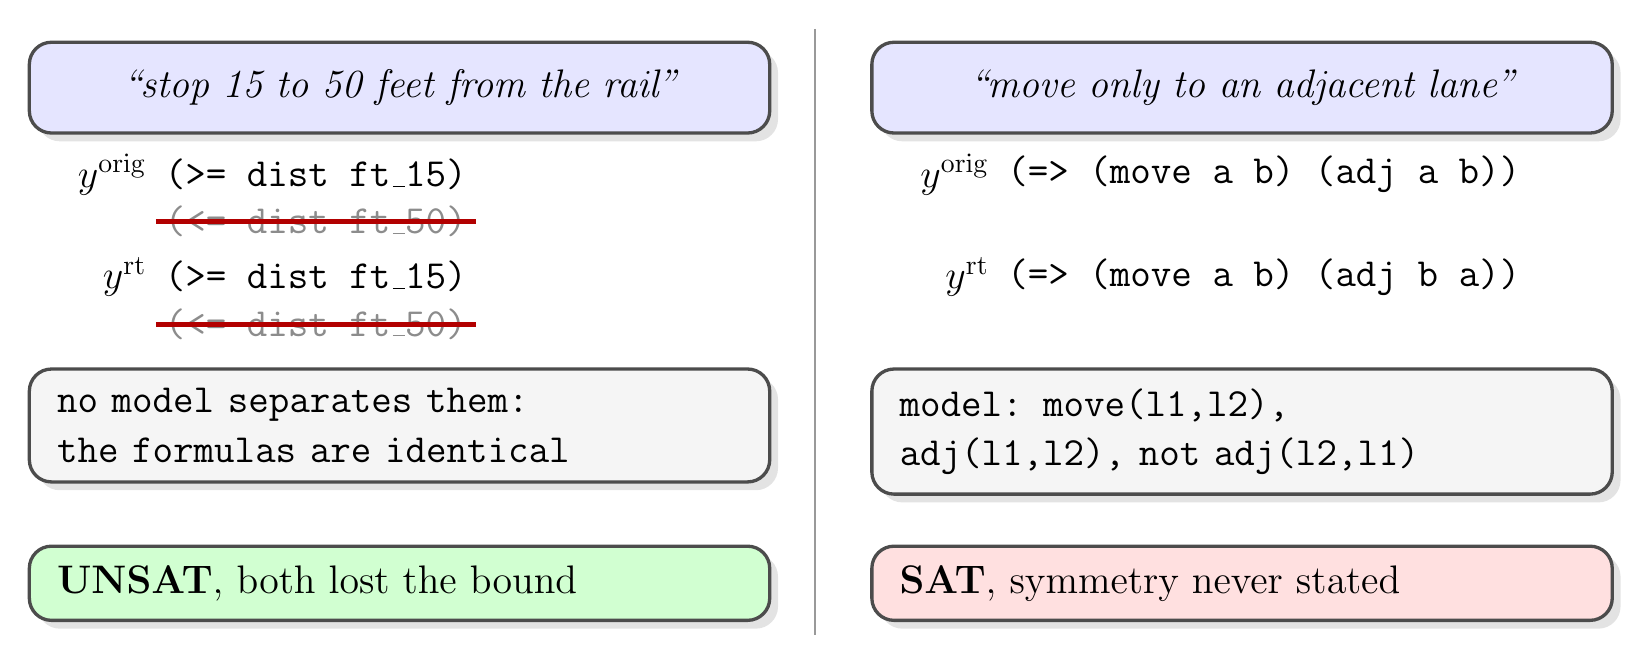
\begin{tikzpicture}[font=\Large,
  card/.style={draw=black!70, line width=1.2pt, rounded corners=8pt, inner sep=10pt,
               drop shadow={opacity=0.22, shadow xshift=3pt, shadow yshift=-3pt}},
  nlcard/.style={card, fill=blue!10, align=center, font=\Large\itshape},
  modelcard/.style={card, fill=black!4, align=left, font=\Large\ttfamily, inner ysep=7pt},
  code/.style={font=\Large\ttfamily, anchor=west, inner sep=1pt},
  dropped/.style={font=\Large\ttfamily, anchor=west, text=black!45, inner sep=1pt},
  lab/.style={font=\Large, anchor=east, inner sep=1pt},
  verdict/.style={card, inner xsep=10pt, inner ysep=7pt, align=left},
]
% ---------------- left: false accept (cards 8.0cm) ----------------
\node[nlcard, text width=8.7cm, anchor=north west] at (0, 3.95) {``stop 15 to 50 feet from the rail''};
\node[lab] at (1.55, 2.25) {$y^{\mathrm{orig}}$};
\node[code] at (1.7, 2.25) {(>= dist ft\_15)};
\node[dropped] (d1) at (1.7, 1.65) {(<= dist ft\_50)};
\draw[red!70!black, line width=1.8pt] ([xshift=-2pt]d1.west) -- ([xshift=2pt]d1.east);
\node[lab] at (1.55, 0.95) {$y^{\mathrm{rt}}$};
\node[code] at (1.7, 0.95) {(>= dist ft\_15)};
\node[dropped] (d2) at (1.7, 0.35) {(<= dist ft\_50)};
\draw[red!70!black, line width=1.8pt] ([xshift=-2pt]d2.west) -- ([xshift=2pt]d2.east);
\node[modelcard, text width=8.7cm, anchor=north west] at (0, -0.2) {no model separates them:\\ the formulas are identical};
\node[verdict, text width=8.7cm, fill=green!18, anchor=north west] at (0, -2.45) {\textbf{UNSAT}, both lost the bound};
% ---------------- divider ----------------
\draw[black!40, line width=0.8pt] (10.0, 4.1) -- (10.0, -3.6);
% ---------------- right: false reject (cards 8.7cm) ----------------
\def\rx{10.7}
\node[nlcard, text width=8.7cm, anchor=north west] at (\rx, 3.95) {``move only to an adjacent lane''};
\node[lab] at (\rx+1.55, 2.25) {$y^{\mathrm{orig}}$};
\node[code] at (\rx+1.7, 2.25) {(=> (move a b) (adj a b))};
\node[lab] at (\rx+1.55, 0.95) {$y^{\mathrm{rt}}$};
\node[code] at (\rx+1.7, 0.95) {(=> (move a b) (adj b a))};
\node[modelcard, text width=8.7cm, anchor=north west] at (\rx, -0.2) {model: move(l1,l2),\\ adj(l1,l2), not adj(l2,l1)};
\node[verdict, text width=8.7cm, fill=red!12, anchor=north west] at (\rx, -2.45) {\textbf{SAT}, symmetry never stated};
\end{tikzpicture}
\end{document}
